\section{Auswertung}
\label{sec:Auswertung}
\subsection{Helmholtzspule}
Die $x$-Skala entspricht der an der Apparatur angebrachten Skala bei der Experimentdurchführung. 
Hierbei war durch $x=0$ die innenliegende Spulenkante der linken Spule gegeben. 
Zur Vereinfachung der Auswertung wurde folgende Verschiebung der Achse vorgenommen, sodass sich idealerweise die Mitte der 
beiden Spulen bei $y=0$ befindet:
\begin{equation*}
    y=x+\frac{b}{2} -\frac{d}{2}
\end{equation*}
Dabei entsprechen $b$ der Spulenbreite und $d$ dem jeweiligen Abstand der Messreihe.

\begin{table}
    \centering
    \caption{Daten der verwendeten Doppelspule und Grundeinstellungen.}
    \label{tab:HH}
    \begin{tabular}{c c c c}
        \toprule
        {Windungszahl je Spule $n$} & {Spulendurchmesser $2R$} & {Spulenbreite $b$} & {Strom $I$}\\
        \midrule
        100 &  $\SI{125}{\milli\m}$ & $\SI{33}{\milli\meter}$ & $\SI{3.03}{\ampere}$\\
        \bottomrule
    \end{tabular}
\end{table}
\begin{table}
    \centering
    \caption{Messreihe mit einem Abstand von $d=R=\SI{62.5}{\milli\meter}$.}
    \label{tab:HH1} %Helmholtz 1
    \begin{tabular}{S[table-format=3.1] S[table-format=2.2] S[table-format=1.3]}
        \toprule
        {$x\,/\,\si{\milli\m}$} & {$y\,/\,\si{\milli\m}$} & {$B\,/\,\si{\milli\tesla}$} \\
        \midrule
        7    & -7.75 & 4.239 \\
        9    & -5.75 & 4.231 \\
        10.5 & -4.25 & 4.234 \\
        12   & -2.75 & 4.260 \\ 
        13.5 & -1.25 & 4.239 \\
        68.5 & 53.75 & 3.003 \\
        69   & 54.25 & 2.960 \\
        70   & 55.25 & 2.891 \\
        75   & 60.25 & 2.666 \\
        80   & 65.25 & 2.445 \\
        85   & 70.25 & 2.219 \\
        90   & 75.25 & 2.018 \\
        95   & 80.25 & 1.839 \\
        100  & 85.25 & 1.662 \\
        \bottomrule
    \end{tabular}
\end{table}
\begin{table}
    \centering
    \caption{Messreihe mit einem Abstand von $d=\SI{104}{\milli\meter}$.}
    \label{tab:HH2} %Helmholtz 2
    \begin{tabular}{S[table-format=3.1] S[table-format=3.2] S[table-format=1.3]}
        \toprule
        {$x\,/\,\si{\milli\m}$} & {$y\,/\,\si{\milli\m}$} & {$B\,/\,\si{\milli\tesla}$} \\
        \midrule
        7     & -28.5 & 3.091 \\
        16    & -19.5 & 2.976 \\
        27    & -8.5  & 2.887 \\
        33.5  & -2    & 2.882 \\
        44    & 8.5   & 2.945 \\
        54.5  & 19    & 3.081 \\
        108.5 & 73    & 2.639 \\
        115   & 79.5  & 2.410 \\
        120   & 84.5  & 2.194 \\
        125   & 89.5  & 2.031 \\
        130   & 94.5  & 1.849 \\
        160   & 124.5 & 1.036 \\
        190   & 154.5 & 0.615 \\
        230   & 194.5 & 0.366 \\
        \bottomrule
    \end{tabular}
\end{table}
\begin{table}
    \centering
    \caption{Messreihe mit einem Abstand von $d=\SI{130}{\milli\meter}$.}
    \label{tab:HH3} %Helmholtz 3
    \begin{tabular}{S[table-format=3.0] S[table-format=3.2] S[table-format=1.3]}
        \toprule
        {$x\,/\,\si{\milli\m}$} & {$y\,/\,\si{\milli\m}$} & {$B\,/\,\si{\milli\tesla}$} \\
        \midrule
        7   & -41.5 & 2.754 \\
        22  & -26.5 & 2.420 \\
        30  & -18.5 & 2.288 \\
        45  & -3.5  & 2.199 \\
        51  & 2.5   & 2.211 \\
        63  & 14.5  & 2.354 \\
        79  & 30.5  & 2.688 \\
        134 & 85.5  & 2.529 \\
        149 & 100.5 & 2.007 \\
        155 & 106.5 & 1.789 \\
        163 & 114.5 & 1.540 \\
        171 & 122.5 & 1.315 \\
        179 & 130.5 & 1.128 \\
        190 & 141.5 & 0.909 \\
        208 & 159.5 & 0.663 \\
        \bottomrule
    \end{tabular}
\end{table}
Mithilfe von Ausdruck \eqref{eqn:2ringe} können die Daten in Abb. \ref{fig:1mess}, \ref{fig:2mess} und \ref{fig:3mess}  mit dem zu erwartenden Verlauf der Flussdichte verglichen werden.
\begin{figure}
    \centering
    %\includegraphics[width=\textwidth]{.../Plots/plot1.pdf}    %es muss kein Verzeichnis nach oben gegangen werden, da das Ausführungsverzeichnis von der make-Datei bestimmt wird
                                                                %bzw. von der main.tex-Datei, wenn man lualatex verwendet
                                                                %außerdem wären es nur 2 Punkte, statt 3 :)
    \includegraphics[width=\textwidth]{Plots/plot1.pdf}
    \caption{1. Messung.}
    \label{fig:1mess}
\end{figure}
\begin{figure}
    \centering
    \begin{subfigure}{0.48\textwidth}
        \centering
        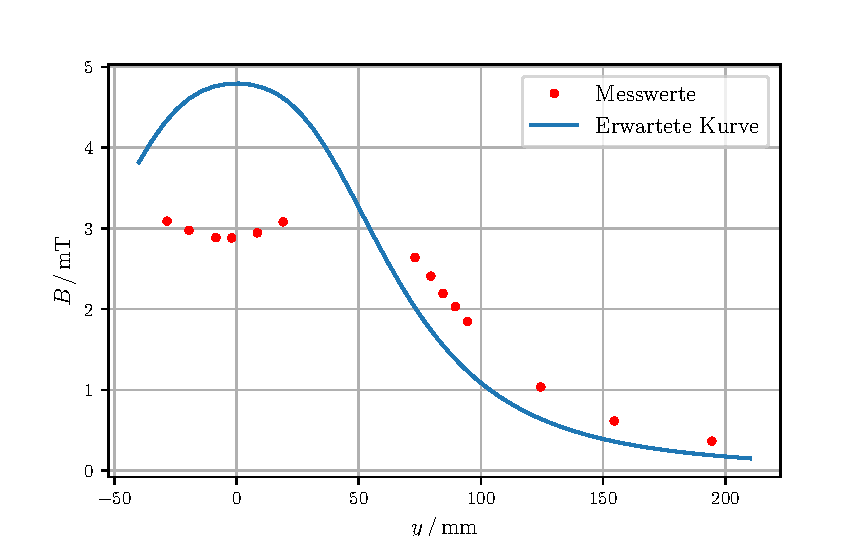
\includegraphics[max width=1.1\linewidth]{Plots/plot2.pdf}
        \caption{2. Messung.}
        \label{fig:2mess}
    \end{subfigure}
    \begin{subfigure}{{0.48\textwidth}}
        \centering
        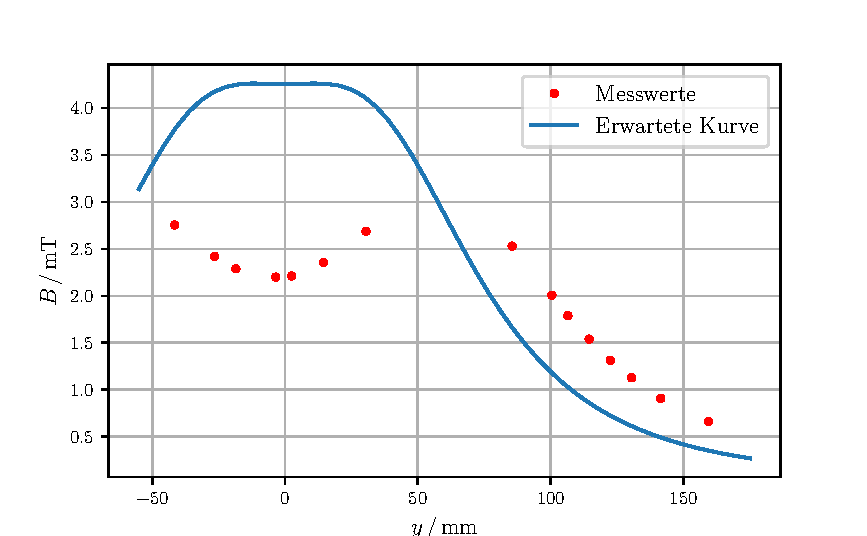
\includegraphics[max width=1.1\linewidth]{Plots/plot3.pdf}
        \caption{3. Messung.}
        \label{fig:3mess}
    \end{subfigure}
    \caption{2. und 3. Messung.}
\end{figure}
\pagebreak
\subsection{Hysteresekurve}
    Gemessen wurden wie erläutert der Strom $I$ durch die Spule und das Magnetfeld im Luftspalt der Spule. 
    Um die Hysteresekurve zu zeichnen, muss die Magnetisierung $M_\text{Fe}$ vom Eisenkern auf das durch die Spule verursachte 
    Magnetfeld $H$ aufgetragen werden. 
    Dafür gelten die Zusammenhänge \eqref{eqn:Magnetisierung} und \eqref{eqn:toroid}: %hier eventuell Referenzen zu den Formeln einfügen, wenn diese bereits in der Theorie erwähnt wurden, und dann mit gather* die Nummerierung wegmachen
    \begin{gather}
        H=\frac{n}{2\symup{\pi}r_T} I \\
        \frac{B_\text{gemessen}}{\symup{\mu_o}} = H+M_\text{Fe}
        \label{eqn:HystereseE}
    \end{gather}
    Die Daten der verwendeten Toroidspule sind:
    \begin{gather*}
        n=595 \\
        r=\SI{13.5}{\centi\meter}
    \end{gather*}
    \begin{table}
        \centering
        \small 
        \caption{Messwerte der Hysteresekurve.}
        \label{tab:Hyst} 
        \begin{tabular}{S[table-format=1.2] S[table-format=1.3] S[table-format=3.0] S[table-format=3.1] S[table-format=3.1]}
            \toprule
            {$I\,/\,\mathrm{A}$} & {$H\,/\,\SI{e3}{\ampere\per\m}$} & {$B_\text{mess}\,/\,\mathrm{mT}$} & {$M_\text{Fe}\,/\,\SI{e3}{\ampere\per\meter}$} & {$B_\text{Fe}\,/\,\mathrm{mT}$} \\
            \midrule
            0.0     & 0         & 0     & 0.0    & 0.0  \\
            1.0     & 0.701    & 148   & 117.0  & 147.1  \\
            2.0     & 1.402     & 335   & 265.1  & 333.2  \\
            3.0     & 2.104     & 440   & 348.0  & 437.3  \\
            4.0     & 2.805     & 508   & 401.4  & 504.4  \\
            5.0     & 3.507     & 561   & 442.9  & 556.5  \\
            6.0     & 4.208     & 603   & 475.6  & 597.7  \\
            7.0     & 4.910     & 638   & 502.7  & 631.8  \\
            8.0     & 5.611     & 668   & 525.9  & 660.9  \\
            9.0     & 6.313     & 698   & 549.1  & 690.0  \\
            8.0     & 5.611     & 677   & 533.1  & 669.9  \\
            7.0     & 4.910     & 656   & 517.1  & 649.8  \\
            6.0     & 4.208     & 632   & 498.7  & 626.7  \\
            5.0     & 3.507     & 604   & 477.1  & 599.5  \\
            4.0     & 2.805     & 569   & 449.9  & 565.4  \\
            3.0     & 2.104     & 524   & 414.8  & 521.3  \\
            2.0     & 1.402     & 460   & 364.6  & 458.2  \\
            1.0     & 0.701    & 332   & 263.4  & 331.1  \\
            0.0     & 0         & 128   & 101.8  & 128.0  \\
            -0.65   & -0.456   &  0    & 0.5    & 0.6  \\
            -1.0    & -0.701   & -71   & -55.8  & -70.1  \\
            -2.0    & -1.402    & -252  & -199.1 & -250.2  \\
            -3.0    & -2.104    & -390  & -308.2 & -387.3  \\
            -4.0    & -2.805    & -482  & -380.7 & -478.4  \\
            -5.0    & -3.507    & -546  & -430.9 & -541.5  \\
            -6.0    & -4.208    & -594  & -468.4 & -588.7  \\
            -7.0    & -4.910    & -634  & -499.6 & -627.8  \\
            -8.0    & -5.611    & -669  & -526.7 & -661.9  \\
            -9.0    & -6.313    & -698  & -549.1 & -690.0  \\
            -8.0    & -5.611    & -679  & -534.7 & -671.9  \\
            -7.0    & -4.910    & -658  & -518.7 & -651.8  \\
            -6.0    & -4.208    & -635  & -501.1 & -629.7  \\
            -5.0    & -3.507    & -607  & -479.5 & -602.5  \\
            -4.0    & -2.805    & -573  & -453.1 & -569.4  \\
            -3.0    & -2.104    & -529  & -418.8 & -526.3  \\
            -2.0    & -1.402    & -464  & -367.8 & -462.2  \\
            -1.0    & -0.701   & -339  & -269.0 & -338.1  \\
            0.0     & 0         & -129  & -102.6 & -129.0  \\
            0.6     & 0.421    & -8    & -6.8   & -8.5  \\
            0.67    & 0.473    & 0     & -0.5   & -0.6  \\
            1.0     & 0.701    & 72    & 56.6   & 71.1  \\
            2.0     & 1.402     & 253   & 199.9  & 251.2  \\
            3.0     & 2.104     & 390   & 308.2  & 387.3  \\
            4.0     & 2.805     & 482   & 380.7  & 478.4  \\
            5.0     & 3.507     & 544   & 429.3  & 539.5  \\
            6.0     & 4.208     & 592   & 466.8  & 586.7  \\
            7.0     & 4.910     & 630   & 496.4  & 623.8  \\
            8.0     & 5.611     & 663   & 521.9  & 655.9  \\
            9.0     & 6.313     & 693   & 545.1  & 685.0  \\
            \bottomrule
        \end{tabular}
    \end{table}
\begin{figure}
    \centering
    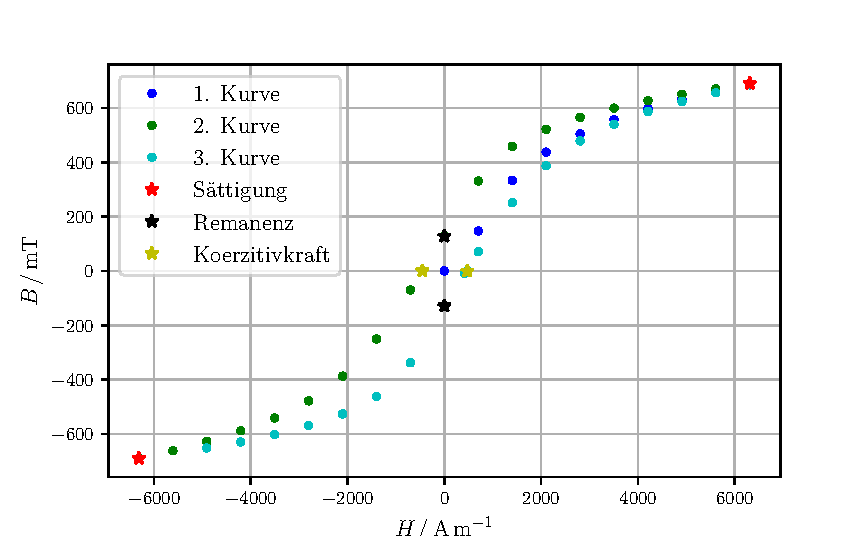
\includegraphics[width=\textwidth]{Plots/plot_Hysterese.pdf}
    \caption{Messwerte der Hysteresekurve.}
    \label{fig:hyst}
\end{figure}
\pagebreak

\subsection{Spulen}
    Die in den Tabellen \ref{tab:kurzSp} und \ref{tab:langSp} ebenfalls aufgeführten $y$-Werte entsprechen einer der $x$-Achse gegenüber verschobenen Achse, sodass
    bei $y=0$ am Anfang der Spule liegt. Das Spuleninnere liegt bei $y<0$.
    \subsubsection{Kurze Spule}
    Verwendet wurde eine Spule mit der Windungszahl $n=3400$, der Länge $l=\SI{8.9}{\centi\meter}$ und dem Durchmesser
    $d=\SI{11.0}{\centi\meter}$. Ein Strom von $I=\SI{0.61}{\ampere}$ wurde angelegt. 
    \begin{table}
    \centering
    \caption{Messwerte der kurzen Spule.}
    \label{tab:kurzSp}
        \begin{tabular}{S[table-format=3.0] S[table-format=2.0] S[table-format=2.2]}
            \toprule
            {$x\,/\,\mathrm{mm}$} & {$y\,/\,\mathrm{mm}$} & {$B\,/\,\mathrm{mT}$}\\
            \midrule
            0   & -96   & 13.71 \\
            15  & -81   & 16.68 \\
            30  & -66   & 18.48 \\
            40  & -56   & 18.81 \\
            50  & -46   & 18.44 \\
            60  & -36   & 17.40 \\
            73  & -23   & 15.02 \\
            87  & -9    & 11.82 \\
            100 & 4     & 8.82  \\
            110 & 14    & 6.90  \\
            121 & 25    & 5.23  \\
            135 & 39    & 3.68  \\
            151 & 55    & 2.52  \\
            \bottomrule
        \end{tabular}
    \end{table}
    \begin{figure}
        \centering
        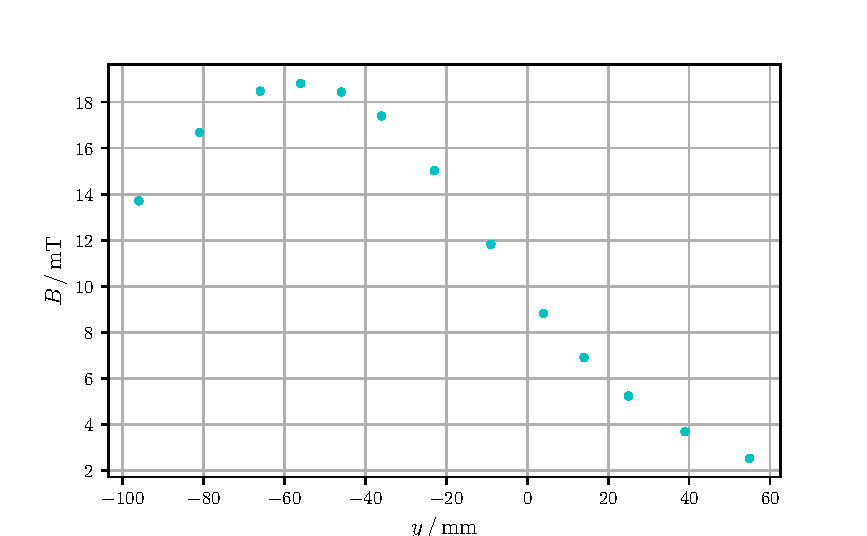
\includegraphics[width=\textwidth]{Plots/plot_kurzSp.pdf}
        \caption{Kurze Spule.}
        \label{fig:kurz}
    \end{figure}
    \pagebreak
    \subsubsection{Lange Spule}
    Die benutzte Spule hat eine Windungszahl von $n=300$ und einen Durchmesser von $d=\SI{41}{\milli\m}$. 
    Der Strom lag bei $I=\SI{1.35}{\ampere}$. Da weder die Länge der Spule in der Versuchsanleitung aufgeführt ist, noch 
    die Länge bei der Versuchsdurchführung von den Experimentierenden aufgenommen wurde, kann der theoretisch zu erwartende 
    Wert der Magnetfeldstärke im Spuleninneren an dieser Stelle nicht berechnet werden. 
    Aus den Messdaten ergibt sich anhand von \eqref{eqn:langespule} eine Länge von etwa $\SI{15}{\centi\m}$, was in Augen 
    der Verfasser ein realistischer 
    Wert für die Spule zu sein scheint.
    \begin{table}
    \centering
    \caption{Messwerte der langen Spule.}
    \label{tab:langSp}
        \begin{tabular}{S[table-format=3.0] S[table-format=2.0] S[table-format=2.2]}
            \toprule
            {$x\,/\,\mathrm{mm}$} & {$y\,/\,\mathrm{mm}$} & {$B\,/\,\mathrm{mT}$}\\
            \midrule
            0   & -79   & 3.076 \\
            5   & -74   & 3.051 \\
            10  & -69   & 3.020 \\
            15  & -64   & 2.977 \\
            20  & -59   & 2.916 \\
            31  & -48   & 2.671 \\
            39  & -40   & 2.318 \\
            47  & -32   & 1.775 \\
            55  & -24   & 1.174 \\
            64  & -15   & 0.680 \\
            70  & -9    & 0.501 \\
            80  & 1     & 0.317 \\
            100 & 21    & 0.177 \\
            \bottomrule
        \end{tabular}
    \end{table}
    \begin{figure}
        \centering
        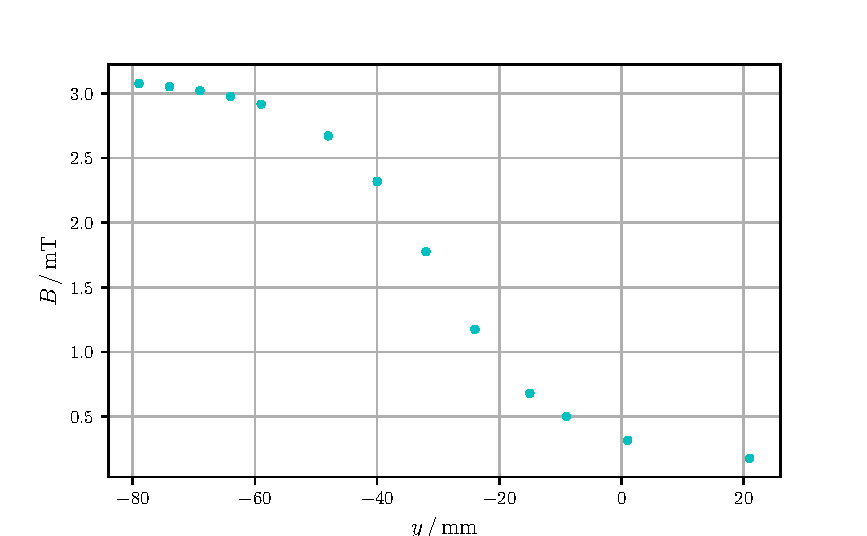
\includegraphics[width=0.85\textwidth]{Plots/plot_langSp.pdf}
        \caption{Lange Spule.}
        \label{fig:lang}
    \end{figure}